\item
    $\frac{\partial\Ab\xb}{\partial\xb}
=
    \frac{\partial\left(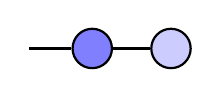
\begin{tikzpicture}[baseline=-0.1ex]
    \tikzset{tensor/.style = {minimum size = 0.5cm,shape = circle,thick,draw=black,inner sep = 0pt}, edge/.style = {thick,line width=.4mm},every loop/.style={}}
    \def\x{6}
    \def\y{0}
    \node[tensor,fill=blue!50!white] (A) at (\x+1,\y) {$\Ab$};
    \node[tensor,fill=blue!20!white] (x) at (\x+2,\y) {$\xb$};
    \draw[edge] (A) -- (x);
    \draw[edge] (A) -- (\x+0.2,\y);
    \end{tikzpicture}\right)}{\partial\left(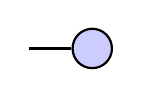
\begin{tikzpicture}[baseline=-0.1ex]
    \tikzset{tensor/.style = {minimum size = 0.5cm,shape = circle,thick,draw=black,inner sep = 0pt}, edge/.style = {thick,line width=.4mm},every loop/.style={}}
    \def\x{6}
    \def\y{0}
    \node[tensor,fill=blue!20!white] (x) at (\x+1,\y) {$\xb$};
    \draw[edge] (x) -- (\x+0.2,\y);
    \end{tikzpicture}\right)}
=
    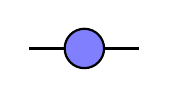
\begin{tikzpicture}[baseline=-0.1ex]
    \tikzset{tensor/.style = {minimum size = 0.5cm,shape = circle,thick,draw=black,inner sep = 0pt}, edge/.style = {thick,line width=.4mm},every loop/.style={}}
    \def\x{6}
    \def\y{0}
    \node[tensor,fill=blue!50!white] (A) at (\x+1,\y) {$\Ab$};
    \draw[edge] (A) -- (\x+0.3,\y);
    \draw[edge] (A) -- (\x+1.7,\y);
    \end{tikzpicture}
=
    \Ab
    $
    
\item 
    $\frac{\partial \xb^\ts\Ab\xb}{\partial\Ab}
=
    \frac{\partial\left(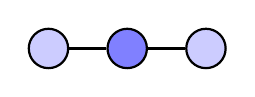
\begin{tikzpicture}[baseline=-0.1ex]
    \tikzset{tensor/.style = {minimum size = 0.5cm,shape = circle,thick,draw=black,inner sep = 0pt}, edge/.style = {thick,line width=.4mm},every loop/.style={}}
    \def\x{6}
    \def\y{0}
    \node[tensor,fill=blue!50!white] (A) at (\x+1,\y) {$\Ab$};
    \node[tensor,fill=blue!20!white] (x) at (\x+2,\y) {$\xb$};
    \node[tensor,fill=blue!20!white] (xt) at (\x,\y) {$\xb$};
    \draw[edge] (A) -- (x);
    \draw[edge] (A) -- (xt);
    \end{tikzpicture}\right)}{\partial\left(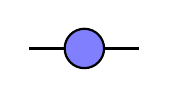
\begin{tikzpicture}[baseline=-0.1ex]
    \tikzset{tensor/.style = {minimum size = 0.5cm,shape = circle,thick,draw=black,inner sep = 0pt}, edge/.style = {thick,line width=.4mm},every loop/.style={}}
    \def\x{6}
    \def\y{0}
    \node[tensor,fill=blue!50!white] (A) at (\x+1,\y) {$\Ab$};
    \draw[edge] (A) -- (\x+1.7,\y);
    \draw[edge] (A) -- (\x+0.3,\y);
    \end{tikzpicture}\right)}
=
    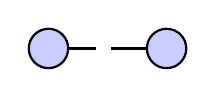
\begin{tikzpicture}[baseline=-0.1ex]
    \tikzset{tensor/.style = {minimum size = 0.5cm,shape = circle,thick,draw=black,inner sep = 0pt}, edge/.style = {thick,line width=.4mm},every loop/.style={}}
    \def\x{6}
    \def\y{0}
    \node[tensor,fill=blue!20!white] (x) at (\x+1,\y) {$\xb$};
    \node[tensor,fill=blue!20!white] (xt) at (\x-0.5,\y) {$\xb$};
    \draw[edge] (x) -- (\x+0.3,\y);
    \draw[edge] (xt) -- (\x+0.1,\y);
    \end{tikzpicture}
=
    \xb\outprod\xb
$
\item 
    $\frac{\partial\tr(\Ab)}{\partial\Ab}
    =
    \frac{\partial\left(
\begin{tikzpicture}[baseline=-0.1ex]
    \tikzset{tensor/.style = {minimum size = 0.5cm,shape = circle,thick,draw=black,inner sep = 0pt}, edge/.style = {thick,line width=.4mm},every loop/.style={}}
    \def\x{6}
    \def\y{0}
    \node[tensor,fill=blue!50!white] (A) at (\x+1,\y) {$\Ab$};
    \draw[edge] (A) to [out=20,in=160, distance=1cm] (A);
    \end{tikzpicture}\right)}
    {\partial\left(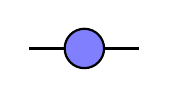
\begin{tikzpicture}[baseline=-0.1ex]
    \tikzset{tensor/.style = {minimum size = 0.5cm,shape = circle,thick,draw=black,inner sep = 0pt}, edge/.style = {thick,line width=.4mm},every loop/.style={}}
    \def\x{6}
    \def\y{0}
    \node[tensor,fill=blue!50!white] (A) at (\x+1,\y) {$\Ab$};
    \draw[edge] (A) -- (\x+1.7,\y);
    \draw[edge] (A) -- (\x+0.3,\y);
    \end{tikzpicture}\right)}
=

\begin{tikzpicture}[baseline=-0.1ex]
    \tikzset{tensor/.style = {minimum size = 0.5cm,shape = circle,thick,draw=black,inner sep = 0pt}, edge/.style = {thick,line width=.4mm},every loop/.style={}}
    \def\x{6}
    \def\y{0}
    \node[draw=none] (A) at (\x+1,\y) {};
    \draw[edge] (A) to [out=20,in=160, distance=1cm] (A);
    \end{tikzpicture}
=
    \Ib
    $
    \item
    $\frac{\partial\Ab\xb}{\partial\Ab}
=
    \frac{\partial\left(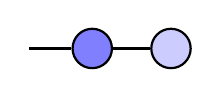
\begin{tikzpicture}[baseline=-0.1ex]
    \tikzset{tensor/.style = {minimum size = 0.5cm,shape = circle,thick,draw=black,inner sep = 0pt}, edge/.style = {thick,line width=.4mm},every loop/.style={}}
    \def\x{6}
    \def\y{0}
    \node[tensor,fill=blue!50!white] (A) at (\x+1,\y) {$\Ab$};
    \node[tensor,fill=blue!20!white] (x) at (\x+2,\y) {$\xb$};
    \draw[edge] (A) -- (x);
    \draw[edge] (A) -- (\x+0.2,\y);
    \end{tikzpicture}\right)}{\partial\left(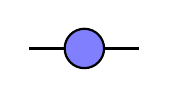
\begin{tikzpicture}[baseline=-0.1ex]
    \tikzset{tensor/.style = {minimum size = 0.5cm,shape = circle,thick,draw=black,inner sep = 0pt}, edge/.style = {thick,line width=.4mm},every loop/.style={}}
    \def\x{6}
    \def\y{0}
    \node[tensor,fill=blue!50!white] (A) at (\x+1,\y) {$\Ab$};
    \draw[edge] (A) -- (\x+0.3,\y);
    \draw[edge] (A) -- (\x+1.7,\y);
    \end{tikzpicture}\right)}
=
    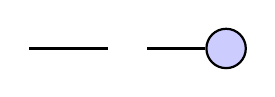
\begin{tikzpicture}[baseline=-0.1ex]
    \tikzset{tensor/.style = {minimum size = 0.5cm,shape = circle,thick,draw=black,inner sep = 0pt}, edge/.style = {thick,line width=.4mm},every loop/.style={}}
    \def\x{6}
    \def\y{0}
    \draw[edge] (\x+2,\y) -- (\x+3,\y);
    \node[tensor,fill=blue!20!white] (x) at (\x+4.5,\y) {$\xb$};
    \draw[edge] (x) -- (\x+3.5,\y);
    \node[draw=none] at (\x+3.25,\y){$\outprod$};
    \end{tikzpicture}
=
    \Ib\outprod\xb
$,
\end{enumerate}
where in the last identity, the result is a third-order tensor.
Theorem~\ref{thm:gradients} applies when the tensor with respect to which the derivative is taken appears only once in the network. The following theorem shows how to handle the case where the tensor appears multiple times.
\begin{theorem}\label{thm:multiple-tensors-gradients}
    Let $\Tt$ be a tensor network where $\Gt$ is a core tensor. If $\Gt$ appears $k$ times in the tensor network of $\Tt$, then $\frac{\partial\Tt}{\partial\Gt}$ is obtained by summing $k$ copies of the tensor network of $\Tt$, where a different occurrence of $\Gt$ is removed in each copy.
\end{theorem}
The following examples illustrate how Theorem~\ref{thm:multiple-tensors-gradients} can be applied.
\paragraph{Examples}
\begin{itemize}
    \item Let $\xb\in\RR^{d}$ and $\Ab\in\RR^{d\times d}$
    \begin{align*}
    \frac{\partial \xb^\ts\Ab\xb}{\partial\xb}
=
    \frac{\partial\left(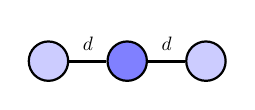
\begin{tikzpicture}[baseline=-0.1ex]
    \tikzset{tensor/.style = {minimum size = 0.5cm,shape = circle,thick,draw=black,inner sep = 0pt}, edge/.style = {thick,line width=.4mm},every loop/.style={}}
    \def\x{6}
    \def\y{0}
    \node[tensor,fill=blue!50!white] (A) at (\x+1,\y) {$\Ab$};
    \node[tensor,fill=blue!20!white] (x) at (\x+2,\y) {$\xb$};
    \node[tensor,fill=blue!20!white] (xprime) at 
    (\x,\y){$\xb$};
    \draw[edge] (A) -- (x)node [midway, above] {\scalebox{0.7}{\dimcolor{$d$}}};
    \draw[edge] (A) -- (xprime)node [midway, above] {\scalebox{0.7}{\dimcolor{$d$}}};
    \end{tikzpicture}\right)}{\partial\left(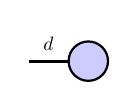
\begin{tikzpicture}[baseline=-0.1ex]
    \tikzset{tensor/.style = {minimum size = 0.5cm,shape = circle,thick,draw=black,inner sep = 0pt}, edge/.style = {thick,line width=.4mm},every loop/.style={}}
    \def\x{6}
    \def\y{0}
    \node[tensor,fill=blue!20!white] (x) at (\x,\y) {$\xb$};
    \draw[edge] (x) -- (\x-0.75,\y)node [midway, above] {\scalebox{0.7}{\dimcolor{$d$}}};
    \end{tikzpicture}\right)}
&=
    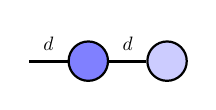
\begin{tikzpicture}[baseline=-0.1ex]
    \tikzset{tensor/.style = {minimum size = 0.5cm,shape = circle,thick,draw=black,inner sep = 0pt}, edge/.style = {thick,line width=.4mm},every loop/.style={}}
    \def\x{6}
    \def\y{0}
    \node[tensor,fill=blue!50!white] (A) at (\x+1,\y) {$\Ab$};
    \node[tensor,fill=blue!20!white] (x) at (\x+2,\y) {$\xb$};
    \draw[edge] (A) -- (x)node [midway, above] {\scalebox{0.7}{\dimcolor{$d$}}};
    \draw[edge] (A) -- (\x+0.25,\y)node [midway, above] {\scalebox{0.7}{\dimcolor{$d$}}};
    \end{tikzpicture}  
    +
    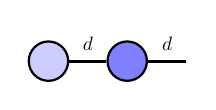
\begin{tikzpicture}[baseline=-0.1ex]
    \tikzset{tensor/.style = {minimum size = 0.5cm,shape = circle,thick,draw=black,inner sep = 0pt}, edge/.style = {thick,line width=.4mm},every loop/.style={}}
    \def\x{6}
    \def\y{0}
    \node[tensor,fill=blue!20!white] (x) at (\x+1,\y) {$\xb$};
    \node[tensor,fill=blue!50!white] (A) at (\x+2,\y) {$\Ab$};
    \draw[edge] (A) -- (x)node [midway, above] {\scalebox{0.7}{\dimcolor{$d$}}};
    \draw[edge] (A) -- (\x+2.75,\y)node [midway, above] {\scalebox{0.7}{\dimcolor{$d$}}};
    \end{tikzpicture}\\  
&=
    \Ab\xb + \Ab^\ts\xb = (\Ab\xb+\Ab^\ts)\xb.
\end{align*}
    \item 
Suppose $\Xb\in\RR^{n\times m},~\Wb\in\RR^{m\times n}$
    \begin{align*}
    \frac{\partial\norm{\Xb\Wb - \Yb}^2_F}{\partial \Wb}
&= 
    \frac{\partial\tr(\Wb^\ts\Xb^\ts\Xb\Wb)}{\partial\Wb}\\
&= 
    \frac{\partial\left( 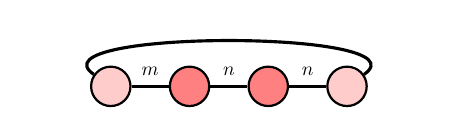
\begin{tikzpicture}[baseline=-0.1ex]
    \tikzset{tensor/.style = {minimum size = 0.5cm,shape = circle,thick,draw=black,inner sep = 0pt}, edge/.style = {thick,line width=.4mm},every loop/.style={}}
    \def\x{6}
    \def\y{0}
    \node[tensor,fill=red!20!white] (Wt) at (\x+1,\y) {$\Wb$};
    \node[tensor,fill=red!50!white] (Xt) at (\x+2,\y) {$\Xb$};
    \node[tensor,fill=red!50!white] (X) at (\x+3,\y) {$\Xb$};
    \node[tensor,fill=red!20!white] (W) at (\x+4,\y) {$\Wb$};
    \draw[edge] (Wt) -- (Xt)node [midway, above] {\scalebox{0.7}{\dimcolor{$m$}}};
    \draw[edge] (Xt) -- (X)node [midway, above] {\scalebox{0.7}{\dimcolor{$n$}}};
    \draw[edge] (X) -- (W)node [midway, above] {\scalebox{0.7}{\dimcolor{$n$}}};
    \draw[edge] (Wt) to [out=145,in=35, distance=1cm] (W);
    \end{tikzpicture}\right)}{\partial\left(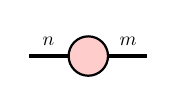
\begin{tikzpicture}[baseline=-0.1ex]
    \tikzset{tensor/.style = {minimum size = 0.5cm,shape = circle,thick,draw=black,inner sep = 0pt}, edge/.style = {thick,line width=.4mm},every loop/.style={}}
    \def\x{6}
    \def\y{0}   
    \node[tensor,fill=red!20!white] (W) at (\x+4,\y) {$\Wb$};
    \draw[edge] (W) -- (\x+4.75,\y)node [midway, above] {\scalebox{0.7}{\dimcolor{$m$}}};
    \draw[edge] (W) -- (\x+3.25,\y)node [midway, above] {\scalebox{0.7}{\dimcolor{$n$}}};
    \end{tikzpicture}\right)}\\
&=
    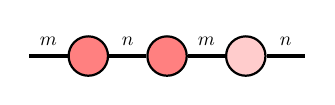
\begin{tikzpicture}[baseline=-0.1ex]
    \tikzset{tensor/.style = {minimum size = 0.5cm,shape = circle,thick,draw=black,inner sep = 0pt}, edge/.style = {thick,line width=.4mm},every loop/.style={}}
    \def\x{6}
    \def\y{0}
    \node[tensor,fill=red!50!white] (Xt) at (\x+2,\y) {$\Xb$};
    \node[tensor,fill=red!50!white] (X) at (\x+3,\y) {$\Xb$};
    \node[tensor,fill=red!20!white] (W) at (\x+4,\y) {$\Wb$};
    \draw[edge] (Xt) -- (\x+1.25,\y)node [midway, above] {\scalebox{0.7}{\dimcolor{$m$}}};
    \draw[edge] (Xt) -- (X)node [midway, above] {\scalebox{0.7}{\dimcolor{$n$}}};
    \draw[edge] (X) -- (W)node [midway, above] {\scalebox{0.7}{\dimcolor{$m$}}};
    \draw[edge] (W) -- (\x+4.75,\y)node [midway, above] {\scalebox{0.7}{\dimcolor{$n$}}};
    \end{tikzpicture}
+
    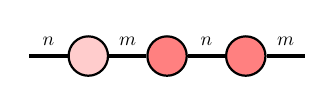
\begin{tikzpicture}[baseline=-0.1ex]
    \tikzset{tensor/.style = {minimum size = 0.5cm,shape = circle,thick,draw=black,inner sep = 0pt}, edge/.style = {thick,line width=.4mm},every loop/.style={}}
    \def\x{6}
    \def\y{0}
    \node[tensor,fill=red!20!white] (Wt) at (\x+1,\y) {$\Wb$};
    \node[tensor,fill=red!50!white] (Xt) at (\x+2,\y) {$\Xb$};
    \node[tensor,fill=red!50!white] (X) at (\x+3,\y) {$\Xb$};
    \draw[edge] (Wt) -- (Xt)node [midway, above] {\scalebox{0.7}{\dimcolor{$m$}}};
    \draw[edge] (Xt) -- (X)node [midway, above] {\scalebox{0.7}{\dimcolor{$n$}}};
    \draw[edge] (Wt) -- (\x+0.25,\y)node [midway, above] {\scalebox{0.7}{\dimcolor{$n$}}};
    \draw[edge] (X) -- (\x+3.75,\y)node [midway, above] {\scalebox{0.7}{\dimcolor{$m$}}};    
    \end{tikzpicture}\\
&=
2\Xb^\ts\Xb\Wb.
\end{align*}
\end{itemize}
We conclude this chapter by presenting several applications of tensor network gradients.
\subsection{Applications}
There is a wide range of applications for tensor network gradients, we highlight two notable examples here. 

